\chapter{Hardware Extension Module Design}

LCS hardware modules typically consist of a controller portion and an extension portion. Welcome to the extension part of hardware module design. To recap, controller boards features an extension connector that contains signal lines to the extension board. This connector provides among other lines an I2C bus, which is the communication bus to elements on the extension boards.

Each hardware module almost certainly has additional requirements. Depending on the module type there will be a great variety of extensions. A good example is the sensor and actor hardware for managing the respective turnouts, signals, and so on. A solution to these family of modules is to use the I2C communication bus and a few more controller lines between controller main board and extensions. Rather than exporting as many as possible pins of the controller via an extension connector, the extension connector presented is hopefully a reasonable compromise when it comes to numbers of pins and capabilities. For complex extension boards with many controller interaction points, a monolithic approach, i.e. controller and extension functionality on one board, would perhaps be the better choice. Such boards could still export the basic functions such as I2C via the extension connector to less complex extension boards for providing additional capabilities. Before we discuss any particular extension board, this chapter will present the hardware and firmware foundation for addressing an extension board.

\section{Requirements}

As with any LCS library part presented, the key goal is to unify and simplify access to an extension board, while still allowing for great flexibility in actual extension board design. We want to be able to connect pretty much any extension board to a main controller, base station and block controller, as well as connecting several extension boards. For example, take the block controller. As shown before, the block controller exports the track power lines and the extension connector. We would like to be able to connect an extension board that implements the track occupancy detectors. We would also like to connect a further extension board that implements the turnout and signal drivers. And of course we want to connect boards then combine one or many of these functions. A key requirement is therefore to communicate to the main controller what is actually connected and how to access the available functions.

\begin{figure}[htbp]
    \centering
    \begin{tikzpicture}[scale=1, transform shape]
        \useasboundingbox (0,0) rectangle (15,6);
        \draw[help lines, gray!50, dashed] (0,0) grid(15,6);

        \node at (3.5, 2.5) {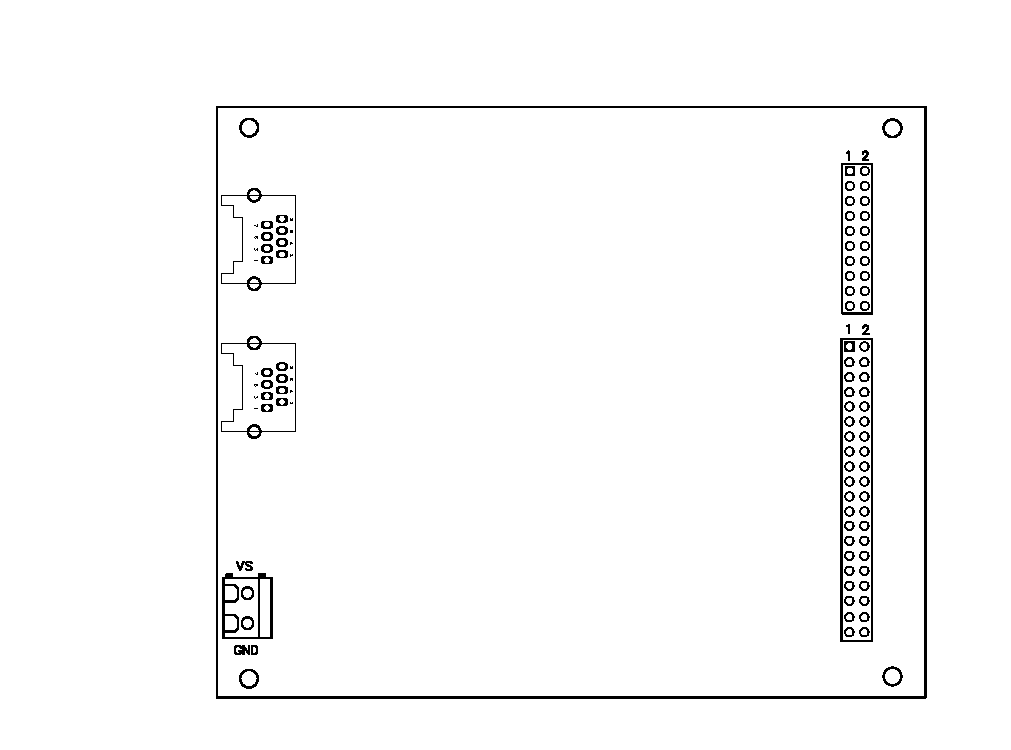
\includegraphics[page=1, width=0.4\textwidth]{./figures/LCS-FP-MAIN-CTRL-Sketch.pdf}};

        \node at (11.5, 2.5) {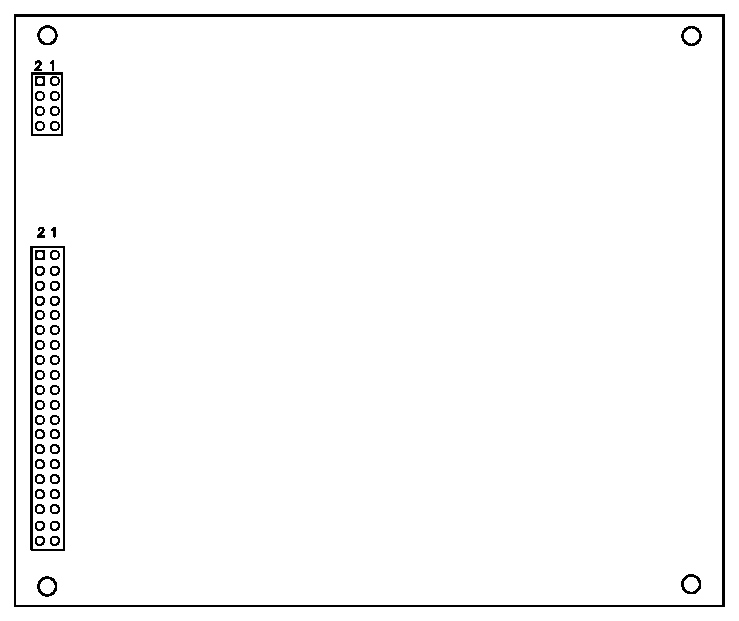
\includegraphics[page=1, width=0.4\textwidth]{./figures/LCS-FP-EXT-L-Sketch.pdf}};

        \node at (3, 5.5) {\textbf{Main Controller}};
        \node at (11, 5.5) {\textbf{Extension Board}};
        \node at (3.5, 4.3) {Track Bus};
        \node at (3.5, 1.7) {Extension Bus};

        \draw[line width=1mm, gray!40, ->] (5, 4.3) -- (11,4.3);
        \draw[line width=1mm, gray!40, ->] (5,1.7) -- (11,1.7);
    
    \end{tikzpicture}
    \caption{Connecting boards}
    %\label{fig:composite-image}
\end{figure}

Typical electronic modules found for digital model railroad control offers configuration options via software and perhaps a set of DIP switches or on board jumpers. As extension boards become more rich in the features they offers and also the combination of more than one board, a methods is needed to uniquely identify and address a board on the extension connectors and a methods to interrogate the capabilities of that particular board.

We already talked about the ability to connect more than one extension board. When this is the case, the order of connected boards should not matter as long as they are uniquely identified. A method is needed for the main controller to automatically identify all extension boards at startup along with their capabilities, ie.e the functions they offer. Other than the methods describing what the board can actually do, the extension board will not have any non-volatile state.

Because of the large variety of extension boards a software layer is needed that unifies how the individual access points such as a digital input or output is accessed by the LCS node firmware. There should be an easy and uniform way to address these endpoints, i.e. there should be some kind of an \textbf{extension library} interface common to all extension boards designed.

The upper layer, i.e. the extension library interface, is complemented by the lower layer which is actually the piece of code that know the extension hardware and translates a higher lever library call into the sequence of actions on the particular extension board. This piece of code will be called \textbf{extension driver}. For each extension board or family of alike boards there is at least one such driver.

\section{Concepts}

To accommodate the requirements, each extension board has to a hardware mechanism that uniquely identifies the board and its capabilities. It is a not a requirement that such a board has processing power or retains any state. This is the responsibility of the controller board. When power is applied to the main controller the reset or restart sequence will attempt to discover all extension boards connected. For this to work, each board has a non-volatile memory structure that describes the board capabilities. And this memory needs to be at a known place, i.e. I2C address, such that this information can be read without knowing any further details. For this purpose, extension boards will have a NVM chip, that contains the board description.

The NVM chip is "programmed" by writing the relevant data to the chip. A write-enable jumper is used to allow writing and then disable all further changes during operation. There is no need for a special programmer, any main controller board can do this via the I2C lines of the extension connector. With using the NV chip, there is no need to have any further DIP switches or alike on the board. In fact, a memory chip allows for even more precise options to configure. And it is cheaper that even a 4-DIP switch.

After programming the NVM chip will contains all information needed to address the extension board functions. Typically, one or more I2C addressable chips are on the board and the NVM tells us what their address is. Combining the chip foxed I2C address portion, the board address portion and the individual chip select portion, an I2C bus unique address is formed. 

The software library can now access a chip. However, chips vary greatly in their functions and how they are controlled by software. A concept is needed to communicate with these chops at  higher abstraction level. Think of a driver in operating systems. A driver offers a set of routines, such as open, read, write and close and takes care of the underlying details how to talk to the physical object. We will go a similar route. There is a high level library, the extension library that offers a high level view of extension board capabilities. Upon node reset and restart, the controller board will query the NVM chips on the extension bod and dynamically configure the driver code for this board.

In addition to the board address a large variety of inputs, outputs and perhaps functions need to be address too. We will call them endpoints. Consider  16-port digital IO chip, such as the MCP23017. It will have 16 IO pins, which we call 16 endpoints. Uniquely identifying an and point is to know the board ID and the endpoint Id on that board. Again, all this information is stored in the NVM  chip at extension board conjuration time. An endpoint could be a variety of things. For example a plan digital output, a servo output, and analog input, and so on. An endpoint could also be a logical entity that groups multiple pins or issue a series of commands to the extension board.

For a new board design, the development process is therefore to define the NVM data that represent the hardware capabilities  and to provide a driver for the board capabilities. From thereon, the firmware designer can use the extension boards with simple but powerful commands. How does this all map to LCS nodes and ports ? Well, the firmware designer has to provide the code that makes the respective driver calls when receiving node and port control commands and events.

\section{I2C Addressing}

An extension board design assumes that the key ICs on the board are I2C addressable chips. As already mentioned, I2C ICs have a fixed I2C address part and a some address bits that can be set by hardware. Most of the I2C chips used in our designs have a four bit fixed address portion and a configurable portion to be supplied via address pins of the chip. We will use the configurable portion to identify the board, from A2 to A1 and reserve the last bit A0 for selecting two chips of the same kind on an extension board.


\begin{longtable}{@{}|l|l|l|l|l|l|l|l|p{0.3\linewidth}|@{}}
    \caption{I2C Chip} \\
    \toprule
    \textbf{IC} & \textbf{A6} & \textbf{A5} & \textbf{A4} & \textbf{A3} & \textbf{A2} & \textbf{A1} & \textbf{A0} & \textbf{Type} \\
    \midrule
    \endfirsthead
    \toprule
    \textbf{IC} & \textbf{A6} & \textbf{A5} & \textbf{A4} & \textbf{A3} & \textbf{A2} & \textbf{A1} & \textbf{A0} & \textbf{Type} \\
    \midrule
    \endhead
    \midrule
    \multicolumn{5}{r}{\textit{Continued on next page}} \\
    \midrule
    \endfoot
    \bottomrule
    \endlastfoot
    \textbf{MCP23017} & 0 & 1 & 0 & 0 & B1 & B0 & x & 16 port DIO \\
    \midrule
    \textbf{PCA9555} & 0 & 1 & 0 & 0 & B1 & B0 & x & 16 port DIO \\
    \midrule
    \textbf{PCA9955} & 1 & 1 & 0 & 1 & B1 & B0 & x & 16 port LED driver \\
    \midrule
    \textbf{PCA9685} & 1 & 1 & 1 & 1 & B1 & B0 & x & 16 port servo driver \\
    \midrule
    \textbf{24AA256} & 1 & 0 & 1 & 0 & B1 & B0 & x & Non volatile memory \\
\end{longtable}%

The PCA 9955 and 9685 have a high number of address selection inputs. This allows to connect more than typically 8 chips on one I2C bus. We will not make use of this capability for now and assign a fixed 4-bit chip I2C address portion.

\section{Multiple Extension Boards}

Now that we talked about I2C address, how does a board get a unique board address without jumpers or alike ? Each board must have a way to contribute to an I2C address its own portion. When an I2C address is sent on the bus, it will have a board ID, this ID is used in the final I2C address. Each extension board features a common set of circuitry for this purpose. The following schematic shows the connectors, the board address generation logic and the NMV chip.

\begin{tikzpicture}[scale=0.9, transform shape]

    \draw[help lines, gray!50, dashed] (0,0) grid( 16,8);
    \node at (8,4) {picture};

\end{tikzpicture}

The design allows for up to four extension boards that can be connected to a controller. Two bits of the I2C address are therefore reserved for the board address. The extension connector pins for analog input 1 and 2 are used to pass on information about the board position in the connecting order. The address generation logic will simply provide the next address value. A "11" input results in a "01", a "01" in "10" and so on. The main controller pins ADC-0 and ADC1 will just not be connected and the pull-up resistors of the first extension board will produce the "00" for the board. The output of the address logic will provide a portion to the  local I2C chip address pins as well as pass it on to the next connected board. Easy and straight forward.

Now, there is always the case to need more pins, i.e. endpoints, that the ICs chosen for the board can deliver in an I2C addressable way. One solution to address the problem could be to spend three pins on the extension connector and implement a serial in/out for chips such as the 74Hc595 ( serial in, parallel out ). This way you could for example realize to drive many output pins, or with an 74HC165 many input pins. Note that this board would need to be connected as the first board to the controller. It is not a requirement for an extension to route through the connector inputs to the output side. As an alternative, there is always the option to use a second controller. Remember, for the layout it is all software in the end.

\section{Extension library}

No LCS concept without a library. This section describes the LCS extension library to access the particular board. As said before, we would like top address each board in a uniform way, regardless what functions it offers. The piece of code that actually manages the board is the extension driver. For each board type to connect to a main controller the firmware needs to have a library loaded for the respective board. The driver exports a set of functions and internally issues the I2C calls to the board hardware. To recap the overall software picture, the firmware layer will make use of the core library and the individual drivers developed for each extension board.

The management of the drivers is part of the core library. This will be presented in a later section. First, let's look at how a driver presents itself to the firmware programmer. To the firmware designer, all boards are accessed to a small set of functions common to all boards using the board Id, an endpoint, which we call \textbf{pad}s.

// ??? code snippets here ?

The core library will locate the board descriptor and the invoke the desired driver routine. That is it. For example, take a write operation. The firmware programmer would simply make a call with the board ID, endpoint ID and data to be written using the core library APIs. The library will locate the board and then call the driver write methods passing the data along. This pretty much sounds like every operations system would do. And in fact, the concept is very similar. While it may sound like an overkill for a simple embedded controller who just wants to make an LED blink, the concept of drivers and a common I/O library allows for building a family of extension boards with common software interfaces and operating concepts. But we also have to acknowledge that it does come with the demand for more processing power. Luckily the Raspberry PI Pico and alike do provide that power. For the Atmega platform that we started with, the limits are reached probably here.

As an idea for the next generation core library, one could imagine to also model the main controller components using the common I/O and driver concept. For example, the NVM on the main board as well as the CAN bus library could just be drivers that you access using the same interfaces as for extension boards. Sounds like, the core library would become more and more a general kind of operating system. Well, maybe one day.

\section{Board Discovery and Setup}

How does a driver know all the details of the board? It has access to the extension board descriptor that was loaded from the board when the board was discovered. Each board has a NVM memory with a fixed i2C address that is computed for the IC base address and the board position. The core library simply tries to access a board using the address. If there is a board, the board descriptor is loaded into the core library data structures and validated. Up to four boards are possible. Once the board is located, the driver method for setting up the board with all initial data for the entry points is invoked. After that, the board is ready to be used using the extension library methods that in turn will just invoke the driver. Note that we could every tome we access the board just read the data needed for accessing a particular board function just read in the portion of the extension board memory. But that would perhaps not result in good performance and since the extension board data does not change, caching it during setup is the better design choice.

\section{Extension Descriptor Memory}

OK, time to present the extension board memory. The LCS core library will simply build the I2C address of the NVM chip on a board and read in the memory data found. The data is rather simple There is a header section which contains information about the board type and how many endpoints are managed. The following code fragment shows the structure of the extension board memory layout.

// ??? header layout ...

// ??? rework text ...

The entry point table is just a simple array with an entry for each in or out channel. For example, a digital IO pin on a general purpose IO extension board would describe each pin with an endpoint descriptor. IN addition. an endpoint could also represent a more complex channel. Take the GPIO board example again. The GPIO chip on such a board, e.g. an MCP23017, would allow to set values on all pins simultaneously. An endpoint could then represent with a 16-bit word all bits to set or read from the chip. It just depends what options the driver will support and what was configured in the extension board NVM.

\section{Extension Board Driver}

Now, we not only know what boards are actually connected but also what software would be required to access the board. We will call this piece of software, essentially a library for each board type, \textbf{extension driver}. The following code fragment will show the common driver class that all actual drivers inherit from. We will see more of actual drivers when discussing a particular extension board implementation.

// ??? code snippet, changed concepts !!

// ??? \textbf{note} what could we do about "real" interrupts from an extension board ?

\section{Utility for writing the NVM}

The structure on each extension board is from the extension library perspective a read-only structure. But of course initially it needs to be filled with valid data. The hardware offers a jumper on the board to enable writing to the NVM chip. Any main controller board could be used to just write to the extension board. This is accomplished with a little utility program or a set of commands implemented in the command line interface of the core library.

// ??? to be decided and implemented. I like the idea for simple commands on the core library level... easiest way to move quickly forward.

\section{Summary}

LCS nodes consist of a main controller board and extension boards. That concept can be found throughout all what is presented in this book. This chapter gave an insight how many different extension boards are connected and managed. We are now read to look at actual extension board implementations in the chapters to come.

